\documentclass[aps,prl,twocolumn,superscriptaddress]{revtex4}
\usepackage{amsmath}
\usepackage{amsfonts}
\usepackage{amssymb}
\usepackage{bm}
\usepackage{dcolumn}
\usepackage{graphicx}
\usepackage[bookmarks,colorlinks]{hyperref}
\usepackage{multirow}

\begin{document}
\title{Theoretical Formalism}

\author{ABC}
\affiliation{National Laboratory of Solid State Microstructures and Department of Physics, Nanjing University, Nanjing 210093, China}
\date{\today}

\maketitle

Most of the previous theoretical works were based on Hubbard model and several mechanisms for the Mott insulator-metal transition have been proposed. However,the picture given by the electron doped Hubbard model cannot explain our experimental observations. For N-site, half-filled Hubbard model in the large U($U/t \rightarrow \infty$) limit, both the spectral weight integral of the LHB and UHB equal to N. Upon single-electron doping, one single-occupied and one empty-occupied state disappeared. The total spectral weight of LHB and UHB are now N-1, and the reduced weight transferred to the bottom of the UHB which is just below the Fermi level as illustrate in Fig. \hyperref[fig:TheoreticalFormalism]{1(a)} \cite{PhysRevLett.67.1035,PhysRevB.48.3916,PhysRevB.48.16857}. The above picture clearly contradicts with our experimental results as additional excitation were observed near the top of LHB.

To have a better understanding of the experimental observations, we adopt the multi-orbital Hubbard model proposed by Shuang Qiao \emph{et al.}, \cite{PhysRevX.7.041054} and use cluster perturbation theory(CPT) \cite{PhysRevLett.84.522,PhysRevB.48.418} to calculate the spectral function as well as density of states of the model Hamiltonian. It is worthy to note that different from chemical substitution or intercalation which actually introduces electron or hole into the crystal, depositing alkali metal atoms onto the surface may not change the electron number but rather refactor the model Hamiltonian instead. Based on the this assumption, we process the multi-orbital Hubbard model with fixed electron number per Star-of-David cluster and the effects of depositing K atoms on the surface are reflected by changing the model parameters.

As we have observed from STM result, the deposited K atoms always located on the center of these SDs, thus it is reasonable to assume that the Potassium cation would reduce the on-site energy difference between $\vert c \rangle$ and $\vert s_{\alpha=1,\dots,6} \rangle$. We studied the case that the averaged number of electron per-SD equals to 13 and the effect of depositing K atoms reflected by decreasing $\mu_c$. From the calculated density of states, the LHB and UHB can be easily identified. The gap between conduction band and LHB is defined as the CDW gap. Most importantly, the additional excitation states does appear near the top of LHB as we have observed from STM experiment. As we can see from Fig. \hyperref[fig:TheoreticalFormalism]{1(c)}, the split-off band has contributions from both $\vert c \rangle$ and $\vert s_{\alpha=1,\dots,6} \rangle$ orbit and the weight of the $\vert c \rangle$ orbit reduces as we decrease $\mu_c$. For N=13 case, the split-off band is half-filled and the total spectral weight of the band equals to 1. However, only the central orbit experiences an effective on-site Coulomb repulsion $U_c$ in our model. The UHB is purely resulted from the Coulomb repulsion experienced by the $\vert c \rangle$ orbit. As the contribution from $\vert c \rangle$ orbit decreased, the spectral weight of UHB would reduce accordingly and reduced weight transferred to LHB.

The seven-orbits Hubbard model is a simplified model which capture the essential physics of the system. However, this does not means that only these seven orbits take effects. When taking these orbits not included in the seven-orbits Hubbard model into consideration, the actual occupation number of these seven orbits may be less than 13. After realising this, we further studied the N=11 case and the effect of depositing K atoms is reflected by increasing the hopping amplitude between $\vert c \rangle$ and $\vert s_{\alpha=1,\dots,6} \rangle$. The density of states calculated using CPT fits well with our experimental data and give a picture completely different from previous works. For small hopping amplitude $t_{sc}$ and appropriate on-site energy difference $\mu_c$, there is a flat band mainly composed of the $\vert c \rangle$ orbit located between the large gap as illustrate is Fig. \hyperref[fig:TheoreticalFormalism]{1(e)}. When we increase $t_{sc}$, the flat band became more dispersive and the conduction band now has contributions from all seven orbits. After taken Hubbard interaction into consideration, the half-filled band split into LHB and UHB and UHB located above the conduction band. The gap observed in experiment is not actually the Mott gap but instead is the gap between LHB and the conduction band.

\begin{figure}
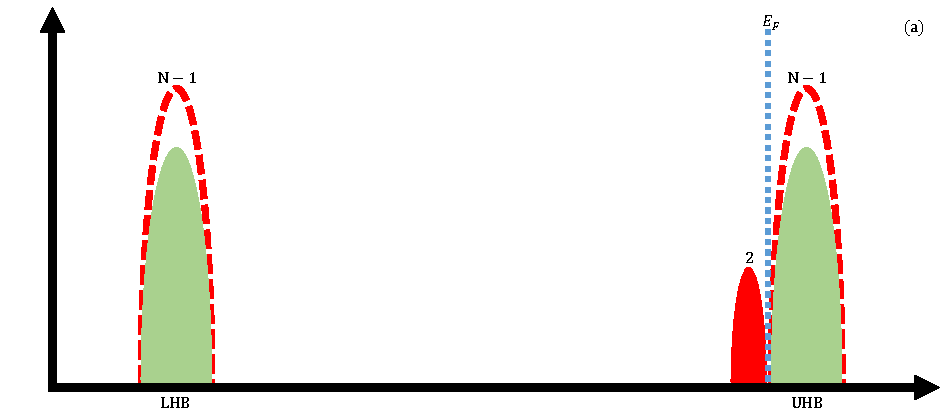
\includegraphics[width=\columnwidth]{AdditionalExcitation.pdf}
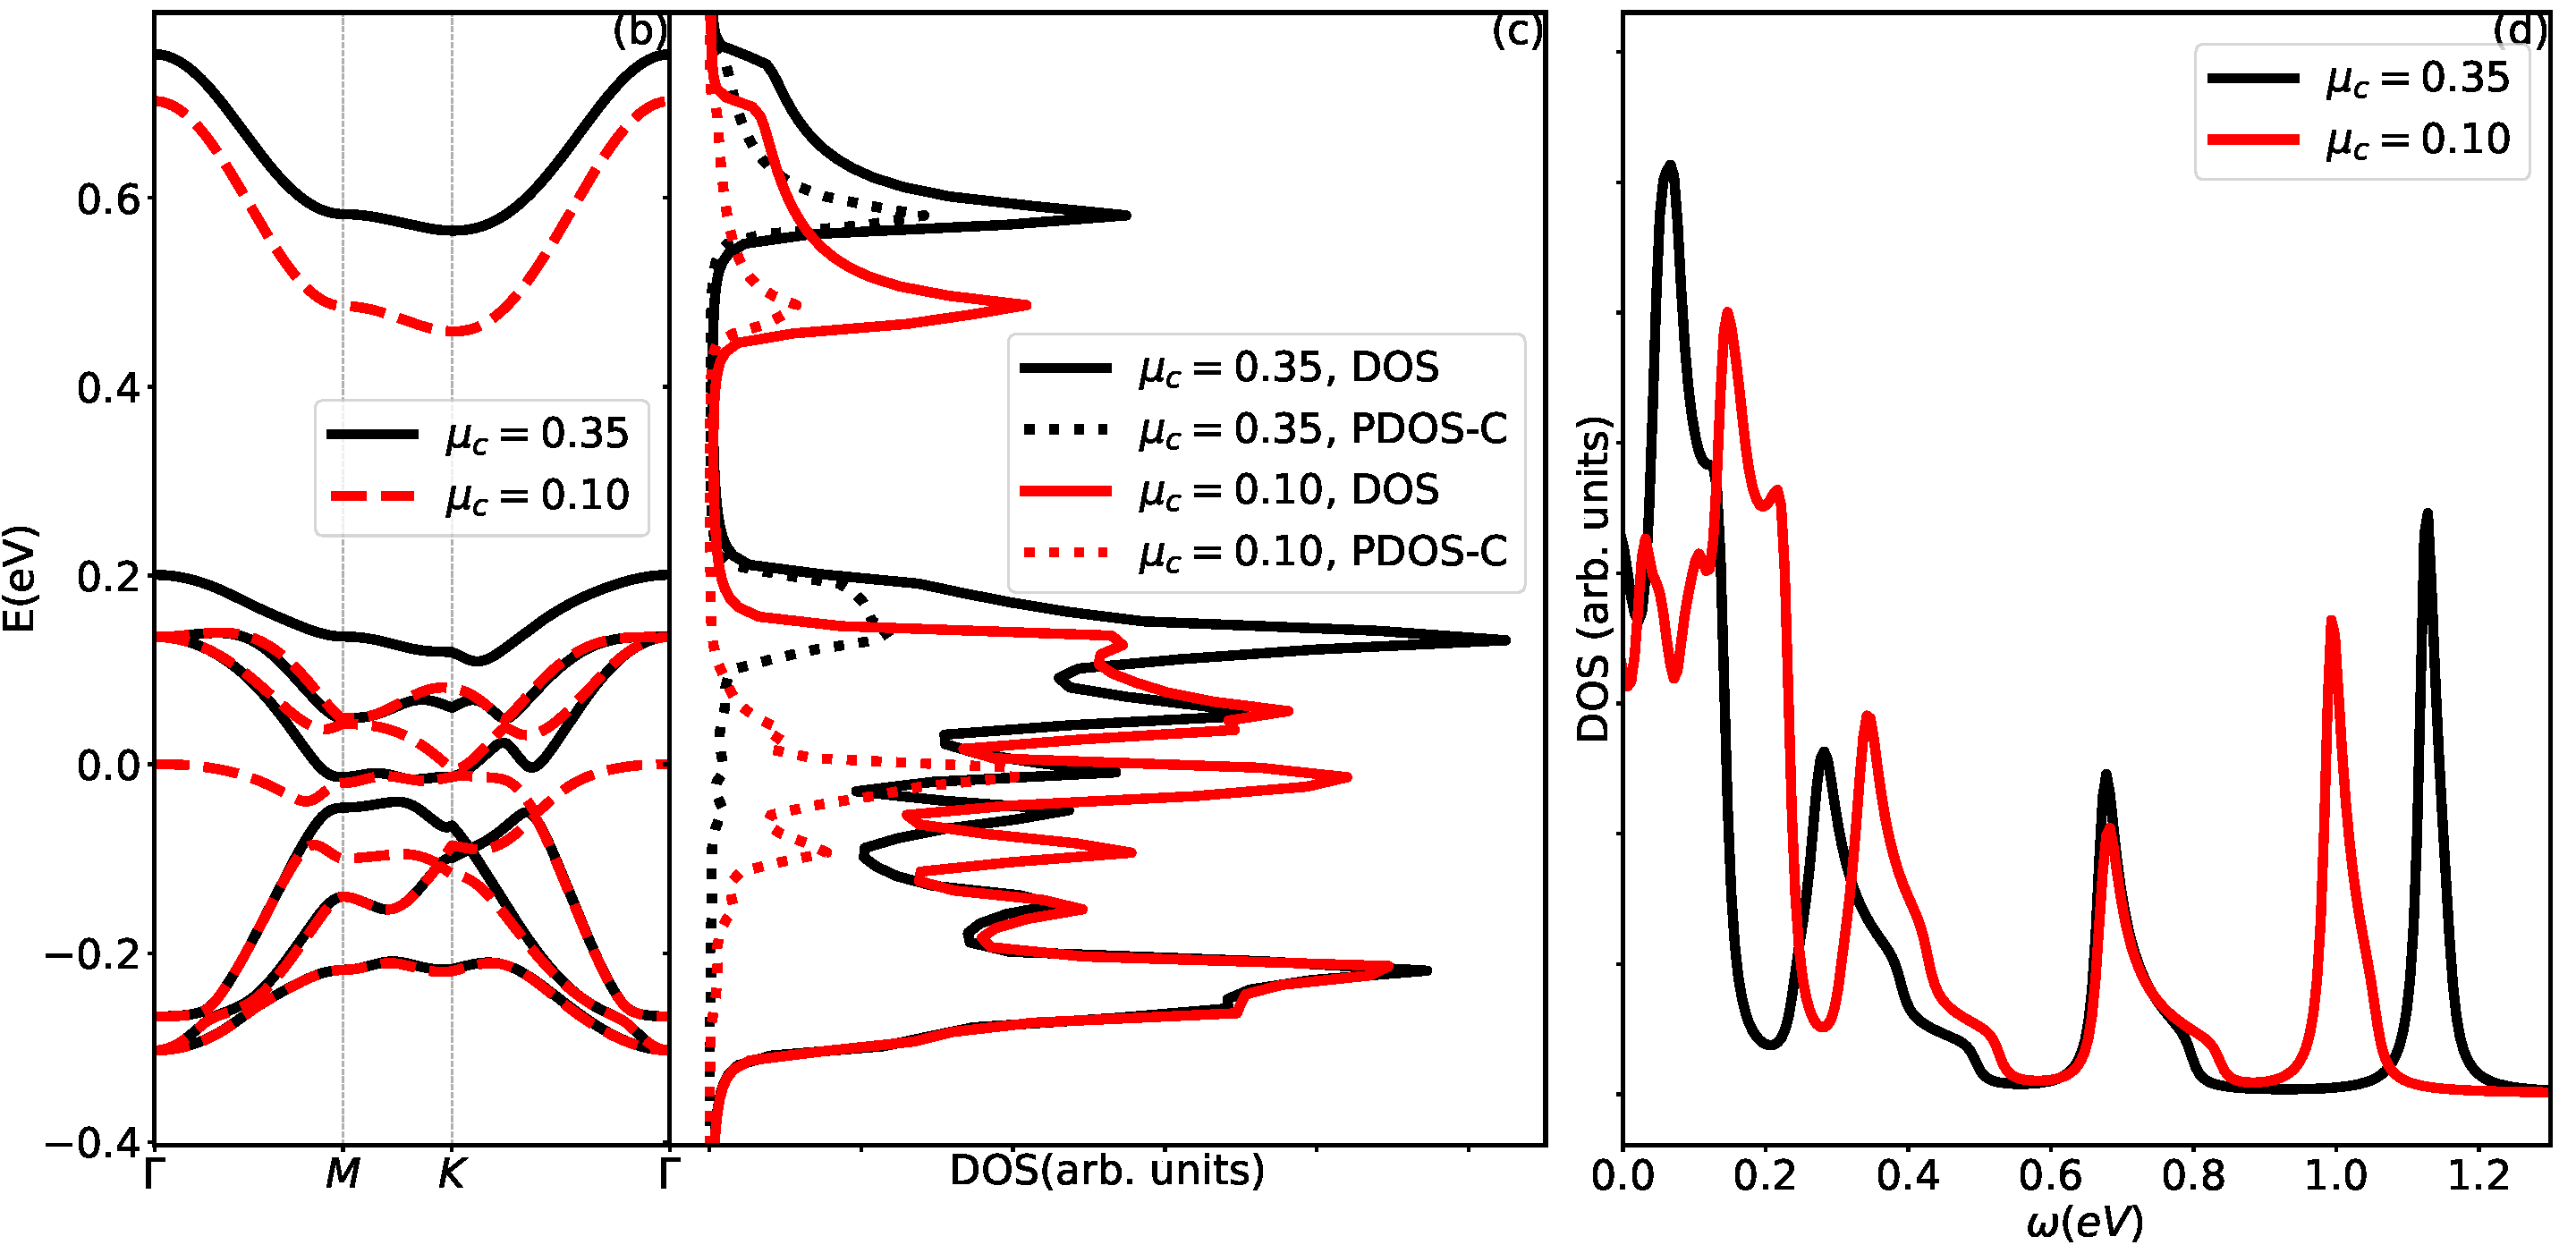
\includegraphics[width=\columnwidth]{ENUM=13.pdf}
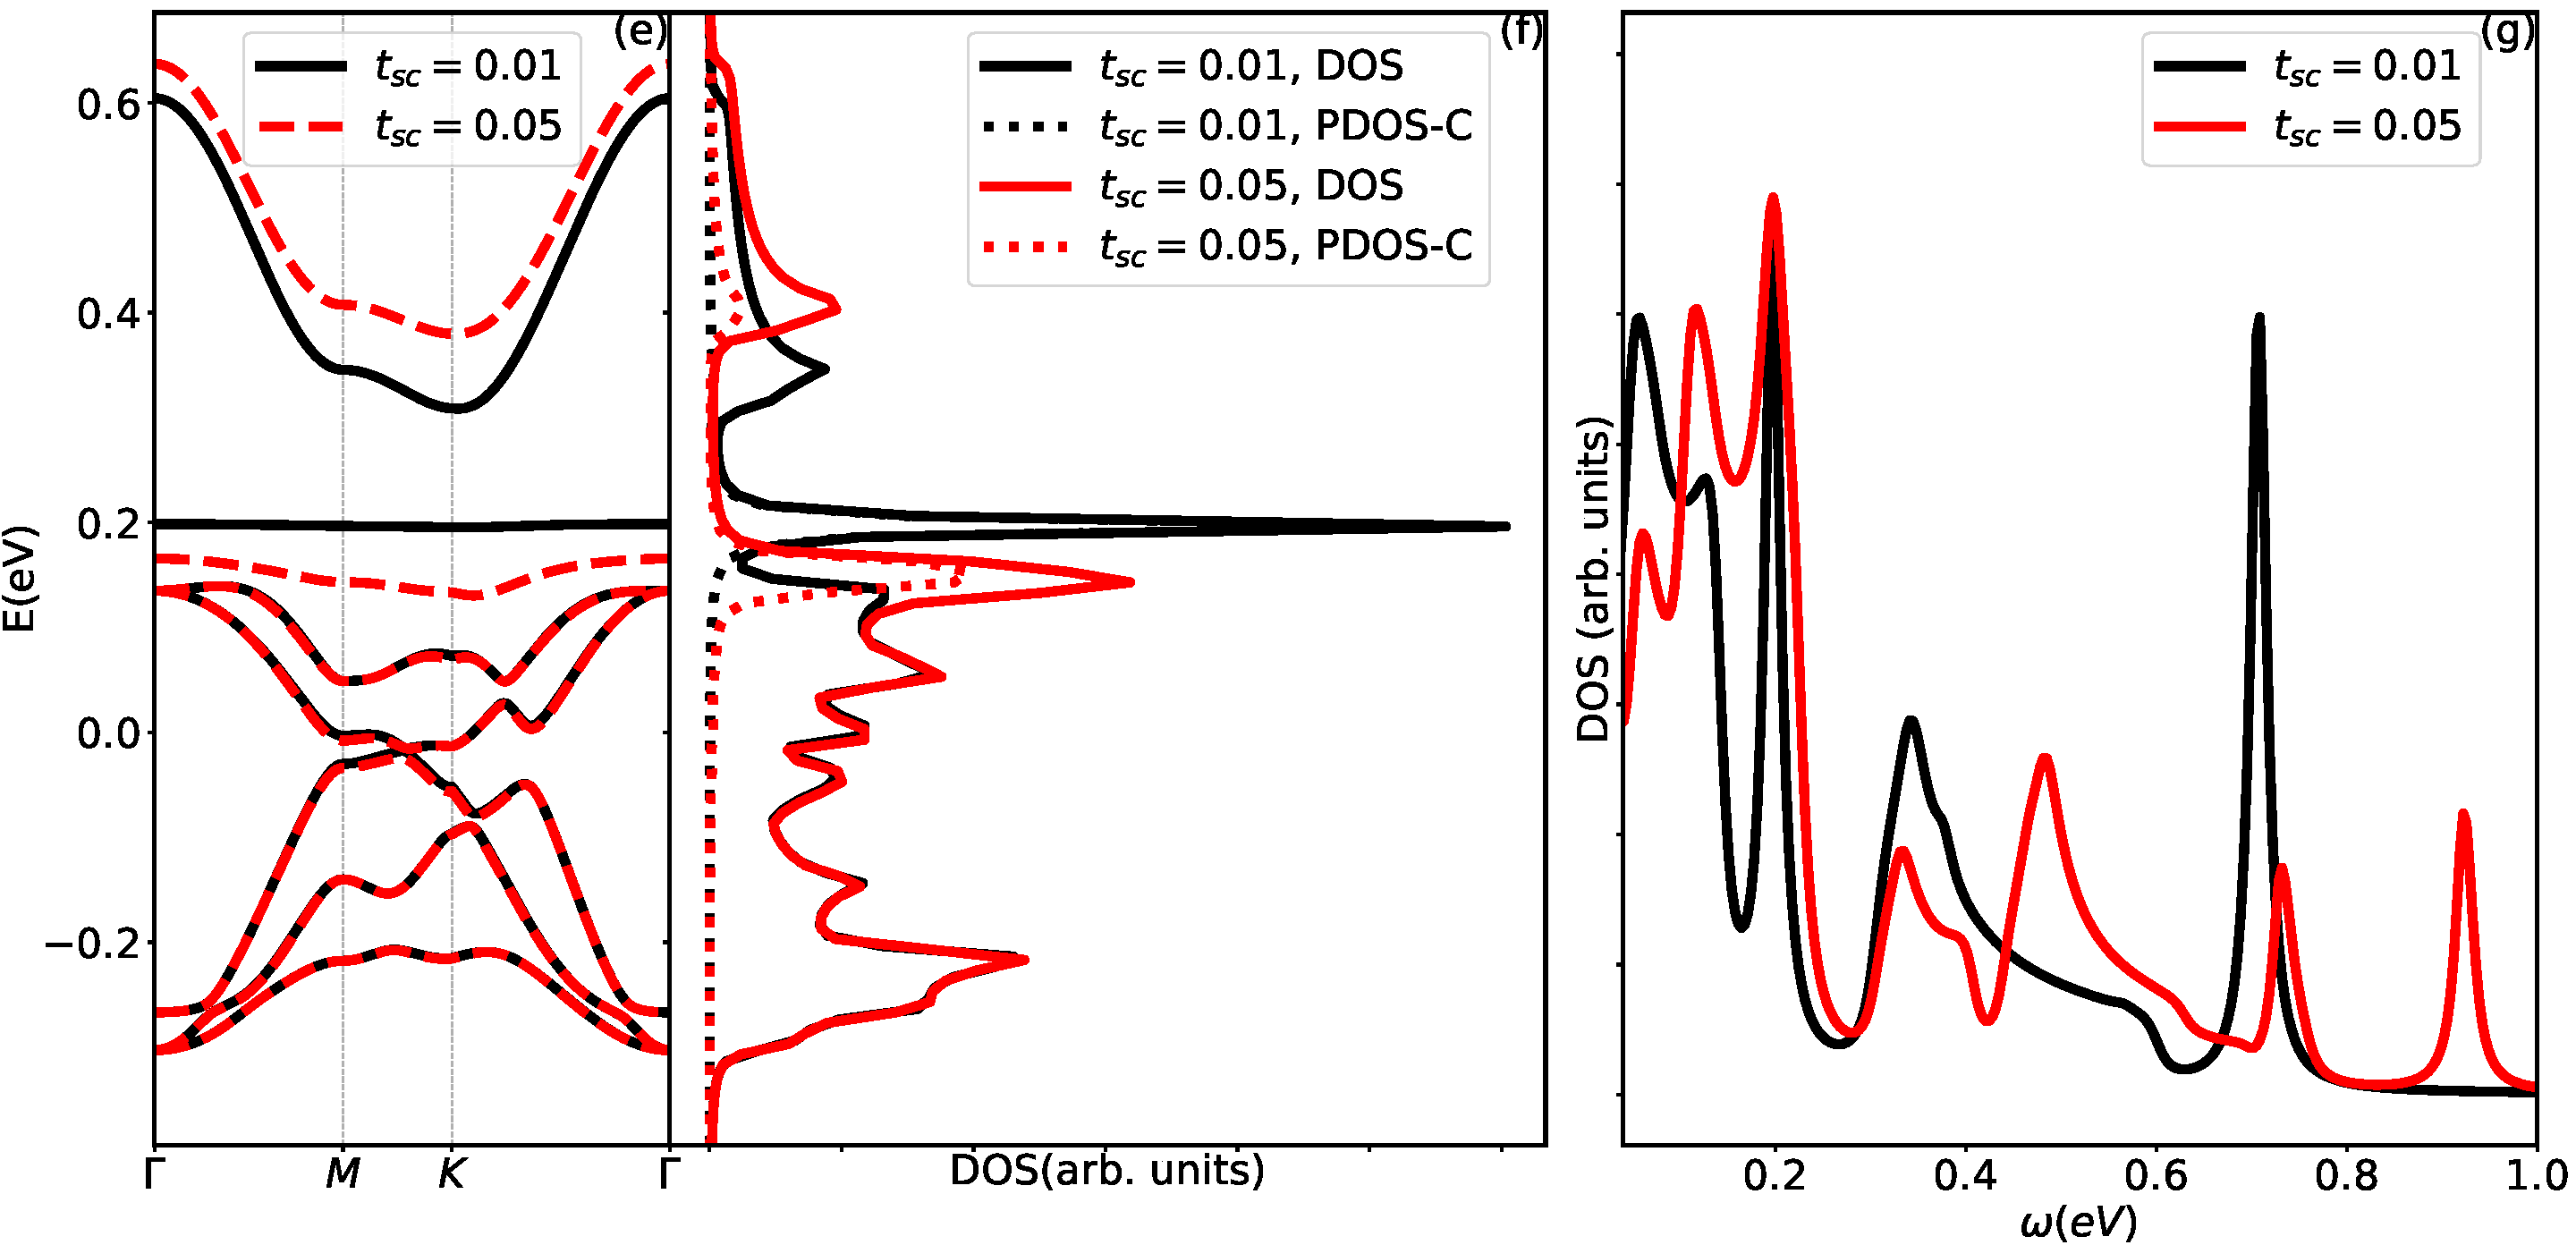
\includegraphics[width=\columnwidth]{ENUM=11.pdf}
\caption{\label{fig:TheoreticalFormalism}
(Color online) (a)Schematic for spectral weight tranfer of the electron doped Hubbard model. (b), (e) Band structure of the tight-binding model. (c), (f) Global and orbital-projected densities of states of the tight-binding model. Solid lines represent global densities of states and dotted lines are the corresponding $\vert c \rangle$ orbital-projected densities of states. (d), (g) Global densities of states for the Hubbard model. For figures (b)-(g), excpet these parameters annotated explicitly, all other parameters are listed in Table \ref{tab:ModelParameters}. The black line correspond to pristine $1\mathrm{T}\text{\ensuremath{-}}{\mathrm{TaS}}_2$, and red line correspond to K atoms deposited case.
}
\end{figure}

\begin{table}
    \caption{\label{tab:ModelParameters}
    Model parameters used in our calculation \cite{PhysRevX.7.041054}
    }
    \begin{ruledtabular}
        \begin{tabular}{ccccc}
            \multirow{2}{*}{Unit(eV)} & \multicolumn{2}{c}{N=13} &  \multicolumn{2}{c}{N=11} \\
            \cline{2-5}
            & Pristine & Deposited & Pristine & Deposited \\
            \cline{1-5}
            $\mu_c$ & 0.350 & 0.100 & 0.200 & 0.200 \\
            $t_{sc}$ & 0.100 & 0.100 & 0.010 & 0.050 \\
            $U_c$ & 0.700 & 0.700 & 0.500 & 0.500 \\
            $t_{ss1}$ & 0.150 & 0.150 & 0.150 & 0.150 \\
            $t_{ss2}$ & 0.091 & 0.091 & 0.091 & 0.091 \\
            $t_{ss3}$ & 0.072 & 0.072 & 0.072 & 0.072 \\
            $t_{ss4}$ & 0.050 & 0.050 & 0.050 & 0.050 \\
            $t_{ss5}$ & 0.042 & 0.042 & 0.042 & 0.042 \\
            $t_{ss6}$ & 0.042 & 0.042 & 0.042 & 0.042 \\
        \end{tabular}
    \end{ruledtabular}
\end{table}

\bibliography{TheoreticalFormalism}

\end{document}
